\documentclass[8.01x]{subfiles}
\begin{document}

\chapter{Week 12}

\section{Lecture 27: Gases and incompressible liquids}

Say we have a vessel containing a fluid, where a fluid is either a liquid \emph{or} a gas\footnote{Or more rarely other states of matter; we will only discuss liquids and gases, however.}. That is, a fluid does \emph{not} refer exclusively to a liquid, unlike colloquial usage of the word.\\
It has an opening of area $A$, where we apply a force $F$.

\begin{center}
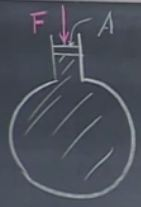
\includegraphics[scale=0.8]{Graphics/lec27_container}
\end{center}

The pressure at the opening is by definition $\displaystyle P = \frac{F}{A}$, measured in pascal (1 Pa = 1 $\text{N/m}^2$).\\
In the absence of gravity, the pressure everywhere inside this vessel in the same; this is known as \emph{Pascal's principle}.

According to Pascal's principle, a pressure enclosed to an enclosed fluid is transmitted undiminished to every point of the fluid, and to the walls of the container.\\
Pressure is a scalar, i.e. it has no direction. Force has a direction, of course, though.\\
The force exerted on the walls of the container must, at all points, be perpendicular to the wall, in a static situation.\\
If there was a tangential component to any such force, that net force would cause movement in the fluid, and we are no longer in a static situation.

As a result of this, for a small area element $\Delta A$ of the container, we can relate the force on that area $\Delta F$ with the pressure:

\begin{equation}
P = \lim_{\Delta A \to 0} \frac{\Delta F}{\Delta A}
\end{equation}

Pascal's principle leads has many interesting consequences, some of which are not very intuitive. First, we shall look at a hydraulic jack.

\subsection{Hydraulic jack}

We have a container, containing a fluid (a practically incompressible liquid); see drawing:

\begin{center}
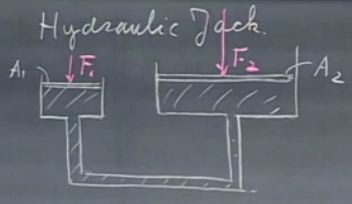
\includegraphics[scale=0.8]{Graphics/lec27_hydraulic_jack}
\end{center}

The left side has a piston of area $A_1$, and the right area a piston of area $A_2$.\\
We apply a downwards force $F_1$ on the left side, and a downwards force $F_2$ on the right side.

According to Pascal's principle, the pressure everywhere in this container is the same. Since the pressure below each piston is that force divided by that piston's area,

\begin{equation}
P = \frac{F_1}{A_1} = \frac{F_2}{A_2}
\end{equation}

when the liquid is not moving. This is also assuming we can neglect gravity, which we will discuss shortly.

We can then design this system such that $A_2/A_1 = 100$. Rearranging the equation,

\begin{equation}
\frac{A_2}{A_1} = \frac{F_2}{F_1}
\end{equation}

We could then have the situation where $F_2 = 100 F_1$, so that we could balance out a very large force with a much smaller one -- similarly to a capstan.

Unlike a capstan, we can use this system to lift very heavy weights easily. We could put a mass of 10 kg on the left piston, and a mass of 1000 kg on the right, and the system would be in equilibrium.\\
This is used, for example, to lift cars. As we expect, if we increase the force $F_1$ a small amount, that piston will go down, which will force the other to go up, lifting the heavy object using a much smaller force.

So how does this work in regards to energy?\\
Well, consider we push the left piston down a distance $d_1$. We displace a volume $d_1 A_1$ of fluid. This fluid has nowhere to go but the right side, where it moves the right piston a distance $d_2$, displacing a volume $d_2 A_2 = d_1 A_1$.

Using the above equation,

\begin{equation}
d_2 = d_1 \frac{A_1}{A_2}
\end{equation}

And since $A_2 > A_1$, we see that we must push $d_1$ down a lot to raise $d_2$ a little. In other words, the work we do, $F_1 d_1$, is equal to the work done at the right side, $F_2 d_2$, assuming no losses.\\
With this ratio, you would have to move the left piston a distance $d_1 = 100$ m, to raise the right piston $d_2 = 1$ m -- rather unpractical if you want to lift a car, for example.\\
However, we can design such a jack so that we can move it a short distance by applying a force with a lever, and then lower it down again, and repeat. This way, we only raise the car (or whatever we are trying to lift) a very small distance at a time, perhaps less than a centimeter, but can repeat the process until we reach the height we want.

\subsection{Pressure due to gravity: hydrostatic pressure}

Until now, we ignored the effect gravity would have on such a system; we will now (essentially for the rest of the lecture) discuss pressure in fluids in the presence of gravity.

Consider a liquid inside some container. We will look at a small ``slab'' of liquid, which is then everywhere surrounded by more of that same liquid.\\
We look at a piece of area $A$, height $\Delta y$ and density $\rho_y$ -- i.e. the density may be a function of $y$.

We have increasing values of $y$ upwards. The call the coordinate at the bottom of the slab $y$, and the one at the top is then $y + \Delta y$.\\
The pressures at the two depths are then $P_y$ and $P_{y + \Delta y}$, respectively.

\begin{center}
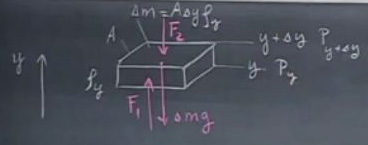
\includegraphics[scale=0.8]{Graphics/lec27_hydrostatic}
\end{center}

The mass of this ``element'' of liquid is $\Delta m = A \Delta y \rho_y$, i.e. simply the volume times the density.\\
Now, what are the forces on this element? First, there is gravity, $\Delta m g$, acting downwards. There is then a force $F_1$ upward, due to the pressure on this element. Keep in mind that the pressure is everywhere perpendicular to a surface -- even on imaginary surfaces like this one.\\
It then also comes in from the top, with force $F_2$. The forces in the horizontal plane all cancel.

For there to be equilibrium, we apply Newton's second law:

\begin{equation}
F_1 - F_2 - \Delta m g = 0
\end{equation}

By definition, $F_1$ is the pressure at that level, times the area, $F_1 = A P_y$. For the same reasons, $F_2 = A P_{y + \Delta y}$.\\
We can then substitute in the expression we had for $\Delta m$, and find

\begin{align}
A P_y - A P_{y + \Delta y} - A \Delta y \rho_y g &= 0\\
P_y - P_{y + \Delta y} - \Delta y \rho_y g &= 0\\
- \Delta y \rho_y g &= P_{y + \Delta y} - P_y\\
- \rho_y g &= \frac{P_{y + \Delta y} - P_y}{\Delta y}
\end{align}

$A$ cancels, and we can then rearrange this a bit, as shown above. Finally, we can take the limit as $\Delta y \to 0$ and we see that what we have is the definition of a derivative,

\begin{equation}
\lim_{\Delta y \to 0} \frac{P_{y + \Delta y} - P_y}{\Delta y} = - \rho_y g \Rightarrow \frac{dP}{dy} = -\rho_y g
\end{equation}

This equation shows us the definition of \emph{hydrostatic pressure}. As the equation tells us, hydrostatic pressure is there because of gravity.

Most liquids are in practice almost completely incompressible, meaning that the density is practically constant, so we can really change $\rho_y$ into $\rho$ above.\\
Even at an ocean depth of 4 km, at pressures of almost 400 times atmospheric pressure (400 atm is about $\SI{4000}{N/cm^2}$) the decrease in volume of water is less than 2\%. Gases, on the other, are often very compressible.

Say we have a liquid in a container, and apply a force on the top (like in the case we had in the beginning of the lecture), we could not get a measurable change in the density using any reasonable force we as humans could apply. With machines, of course, we absolutely could compress it.

If we hit an air-filled plastic pillow with a sledgehammer, the air would act as a cushion. If we instead hit a marble floor, the pressure on the sledgehammer (and on the floor) would be way higher than that of the pillow, since the marble floor is almost completely rigid and incompressible, so this ``cushioning'' effect is gone.

Now consider two metal paint cans. One is completely filled with water (with no air at all inside), while another is filled with air (at atmospheric pressure).\\
If we hit these two cans with a sledgehammer, there would again be a cushion effect one the one filled with air, while the force (and pressure) on the one filled with water would be much higher.

If we now fire a bullet into these containers instead, what happens? The area where the bullet hits is very small, but the force is clearly very high. With these two effects in combination, the pressure will be extremely high.\\
Pascal's principle says that the pressure will propagate undiminished in the fluid.\\
In the one filled with air, there is not much of a problem: the air is glad to change its volume/density to take care of this.\\
In the one filled with water, however, the pressure is extremely high, and the can may will explode due to the extreme pressure on the sides of the can, as the water won't compress any noticeable amount.

\subsection{Pascal's law}

From now on, we will assume that liquids are completely incompressible.\\
With that in mind, we can now treat $\rho$ as a a constant, and calculate the pressure change as a function of a change in depth, via separation of variables. Again, considering that $+y$ is upwards, and $y_2 > y_1$ (below),

\begin{align}
\frac{dP}{dy} &= - \rho g\\
\mathop{dP} &= - \rho g \mathop{dy}
\end{align}

We can integrate both sides, from $y_1$ to $y_2$ and $P_1$ (pressure at $y_1$) to $P_2$ (pressure at $y_2$) respectively. $g$ is also constant, so the integrals are just the integrals of the differentials themselves (think of it as $\int_a^b 1 \mathop{dx}$).

\begin{align}
\int_{P_1}^{P_2} \mathop{dP} &= - \rho g \int_{y_1}^{y_2}\mathop{dy}\\
P_2 - P_1 &= -\rho g(y_2 - y_1)
\end{align}

Equivalently, we can multiply both sides by $-1$ and get

\begin{equation}
P_1 - P_2 = \rho g(y_2 - y_1)
\end{equation}

which you may or may not prefer.\\
This result is known as \emph{Pascal's law}.

Consider a strange-shaped vessel containing a liquid:

\begin{center}
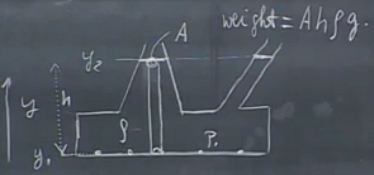
\includegraphics[scale=0.7]{Graphics/lec27_strange_container}
\end{center}

According to Pascal's law, the pressure at the bottom must be the same, at all points along the bottom (assuming the liquid is static).\\
However, consider the point just below the marked cylinder: the water column has a weight $A h \rho g$ -- its volume $A h$, times the density $\rho$ which gives its mass, times $g$ which gives its weight. The pressure at the bottom is this weight divided by the area, i.e $\rho h g$.

However, the pressure just below that column must be exactly the same as the pressure in the corner, where the water column above is much smaller. Not that intuitive.\\
If we think of it in terms of requiring no net force for a static situation, it does make sense, but from the perspective of weight, it does not.

What is the pressure difference due to gravity for a water column that is 10 meters high?

Well, using $P_2 - P_1 = \Delta P$ and $y_2 - y_1 = \Delta y$ we find, using the previous formulas, $|\Delta P| = \rho g \Delta y$.\\
$\rho$ for water is $\SI{1}{g/cm^3} = \SI{1000}{kg/m^3}$. Using $g = \SI{10}{m/s^2}$ and $\Delta y = \SI{10}{m}$, we find $\Delta P = 10^5$ Pa, which incidentally is very close to 1 atmosphere of pressure (i.e. the pressure the air exerts on us, all the time), which is defined as 101325 Pa; more on that soon.\\
This is a very useful thing to remember: there is an additional 1 atm of pressure for each 10 meters you go down in water.

\subsection{Atmospheric pressure and barometers}

``We live at the bottom of an ocean of air'', as the professor says.

Unlike liquids, the density of air changes noticeable with altitude (clearly: as we go up, sooner or later, the density is almost exactly zero, out in space, and the change is gradual), so we can't do the very simple integration we did earlier with the $\rho$ of air.\\
We can weigh it, though. Look back to the case of the strange-shaped vessel with water: the pressure at the bottom, below a column of water stretching all the way up, was the same as the weight of that column, divided by the area.

In the same way, if we weigh a column of air stretching up to the edge of the atmosphere, we would measure a weight of approximately 10 N per square centimeter. There are 10000 square centimeters in a square meter, so the pressure is about $10^5 \text{N/m}^2 = 10^5 \text{ Pa}$.

More exactly, atmospheric pressure is, as mentioned earlier, defined to be exactly 101325 Pa. It varies with the weather, altitude, etc., but is often relatively nearby. In my case, living within 25 m of sea level, I find it rare to look at a barometer and see a value outside the range 970-1030 hPa (i.e. 97000-103000 Pa).

If we hold out our hands, we feel a force equivalent to about 150 kilogram-force or kgf\footnote{1 kgf = 1 kg times $\SI{9.80665}{m/s^2}$; the unit is used so that we can talk about forces in terms of kilograms, which are more familiar in daily usage than newtons.} pushing downwards.\\
However, there is also a force of almost exactly equal magnitude pushing up on the hand's underside, as well as horizontal forces in many directions. All of these forces are, as mentioned earlier, exactly perpendicular to the hand, if the air is not moving.

We can measure the atmospheric pressure in a rather different way. We emerge a hose completely in a liquid of known density, and block off the the top end. The liquid will stay inside the tube, so that it is filled all the way, up to a certain height. For water, this height is about 10 meters; at that point, the liquid ``lets go'' and the very top of the tube will contain a vacuum.

Consider now instead a glass tube instead of a hose, and mercury instead of water. Mercury is way denser than water, so the height required will also be way less than the 10 meters required for water.

\begin{center}
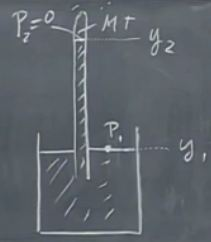
\includegraphics[scale=0.8]{Graphics/lec27_barometer}
\end{center}

(MT means empty, nothing more; I'm not sure why it is written in short.)

$P_1$ is clearly just the atmospheric pressure, since it is in direct ``contact'' with the outside air.\\
A distance $y_2 - y_1 = h$ above, the pressure is $P_2 = 0$, since there is a vacuum.

We have the formula $P_1 - P_2 = \rho g(y_2 - y_1)$, but since $P_2 = 0$ and $P_1$ is the atmospheric pressure, using the definition of $h$, we have

\begin{equation}
P_{atm} = \rho g h
\end{equation}

where $h$ then is the height of the column of mercury. This device is known as a \emph{barometer}.\\
Using $P_{atm} = 101325$ Pa as an example (it can clearly differ), combined with $g = \SI{9.81}{m/s^2}$ and $\rho = \SI{13.6e3}{kg/m^3}$, we find that the height of the column will be about 760 mm.\\
Because mercury barometers were quite common in the past, this pressure is often referred to as 760 mmHg. Other pressures are also measured in mmHg -- ``millimeters of mercury''; blood pressure is almost always measured in mmHg (the ``golden standard'' of approximately 120 over 80, for example, is measured in mmHg).

For water, using the same formula, we see that the column would then have to be about 10 meters high (as mentioned earlier), which is impractical, yet possible.

\subsection{Submarines and hydrostatic pressure}

Construction of the world's first submarine is usually credited to Dutchman Cornelius van Drebbel, as early as 1622. He not only built it, but successfully operated it at a depth of 5 meters, where the hydrostatic pressure is about 0.5 atmospheres. Add to that the atmospheric pressure of 1 atmosphere, and you get a total pressure of 1.5 atm at that depth.

Since he had 1 atmosphere of air inside, to breathe, the pressure differential is then 0.5 atmospheres, equivalent to about 50 kPa or 5000 kgf per square meter acting on the outside; very impressive for the time.

The professor mentions that modern submarines have gone down to at least a 900 meter depth, meaning approximately 90 atmospheres of hydrostatic pressure, but for some reason made no mention of the manned descents into the Challenger Deep (once in 1960, once in 2012; the latter was after the lecture was recorded, however) to a depth of about 10920 meters! The pressure down there is over \emph{a thousand} atmospheres, equivalent to over $10^8$ Pa, or equivalent to having over ten thousand metric tons of mass on each square meter of the outside, in Earth's gravitational field that is. The fact that this is not only possible, but was done even before the first moon landing, amazes me quite a lot.\\
These descents are not done in regular submarines, of course, but they are still man-made vessels that can withstand such absurd pressures.

The professor demonstrates what a ``small'' pressure difference of 0.5-1 atm can do to an object, by sucking the air out of a paint can. There will then be an underpressure inside the can, i.e. the pressure is larger outside than inside.

Long before the pressure difference is 1 atm (i.e. before there is a vacuum inside the can), it has already crumpled up quite a lot. Based on what happens, it's fairly safe to say that this paint can wouldn't survive at a 5 meter depth, if filled with 1 atmosphere of air and then hermetically sealed. 

Now, consider what happens when we go scuba diving. Could we snorkel at a 10 meter depth? Far from it, actually!\\
The air in our lungs would be at 1 atm, connected to the surface via a snorkel (or a simple hose, etc). The pressure on our chests from the outside would be about 2 atm, however, since there is a hydrostatic pressure of 1 atm in addition to the atmospheric pressure of the air at the surface.

Since 1 atm is about 100 kN per square meter, or 10 tons worth of weight, raising your chest to breathe in is absolutely impossible under these conditions. If you can't breathe with a car standing on your chest, how could you breathe with an equivalent hydrostatic force of the same magnitude pushing in on you? (Based on a chest size of about a tenth of a square meter, or so, the force will be about one ton's worth of weight at $g$.)\\
So at what depths \emph{could} we snorkel?

Well, to answer the question, we would need to know approximately what sort of underpressure we can have in our lungs, and still be able to breathe in. It seems reasonable, but tough, that we could perhaps lift a 100 kg weight laying on our chests, using only our lungs. I doubt that it's easy, but it's probably doable, at least for some humans.\\
Given a chest area of 0.3 times 0.3 meters, or 0.1 square meters, this is equivalent to a pressure of about $\displaystyle \frac{(\SI{100}{kg})(\SI{10}{m/s^2})}{\SI{0.1}{m^2}}$, or about 10000 Pa.\\
That is, the outside pressure cannot be more than 10000 Pa greater than atmospheric pressure; that is about 0.1 atmospheres.

At what depth is the hydrostatic pressure 0.1 atm? With the rule of 1 atm per 10 meters, this is at about 1 meter, or so. So a roughly calculated answer is than snorkeling at a depth greater than 1 meter is essentially impossible.\\
We will look at this in more detail now.

By the way, the way divers get around this is to have pressurized breathing gas. That is, the air in their lungs is at about the same pressure as the water outside.

\subsection{Manometers}

A manometer is a very simple device that can be used to measure pressure. We have a U-shaped tube, plastic in this case, which is partially filled with water.

\begin{center}
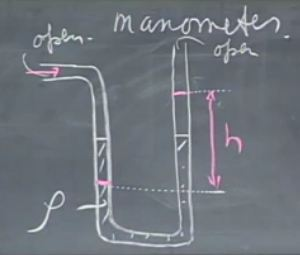
\includegraphics[scale=0.8]{Graphics/lec27_manometer}
\end{center}

By blowing (or sucking) on one end, we can measure the height difference in the liquid, and calculate the amount of underpressure/overpressure we managed to produce in our lungs.\\
Call the top height $y_2$ with pressure $P_2$, and the bottom $y_1$ with pressure $P_1$, we have

\begin{equation}
P_1 - P_2 = \rho h g
\end{equation}

$P_2$ is at atmospheric pressure, since it is connected to the outside world. Therefore, solving for $P_1$ and making a substitution,

\begin{equation}
P_1 = \SI{1}{atm} + \rho h g
\end{equation}

So we can measure the amount of pressure we can generate above or below the atmospheric pressure. We call that overpressure and underpressure, respectively.\\
If you have ever measured the pressure in a car's tires, that is done by an overpressure gauge.

If we use water in the manometer, the height difference it shows is equal to the depth at which we could snorkel (for a short amount of time, at least), since 1 meter on the manometer means we can generate an overpressure of 0.1 atm, and the hydrostatic pressure at such a depth also is 0.1 atm.\\
The hard part of snorkeling is breathing \emph{in}, though -- out is easy, since your lungs are compressed from the outside. In other to find out out maximum snorkeling depth, we need to measure the maximum \emph{underpressure} we can produce, i.e. when sucking.

The professor then demonstrates this, and then demonstrates an interesting feat: drinking with a ``straw'' that is much, much longer than the 1 meter he could manage with the manometer. Exactly how it's done is not explained.

\section{Lecture 28: Hydrostatics, Archimedes' principle, and fluid dynamics}

We will now look at how objects float.\\
Say we have a cylinder of end-cap area $A$ and length $\ell$, and therefore volume $A \ell$. It has a uniform density $\rho$, and therefore a mass $M = A \ell \rho$.\\
The cylinder is in a liquid of density $\rho_{fl}$, and a height $h = y_2 - y_1$ of the cylinder is submerged.

\begin{center}
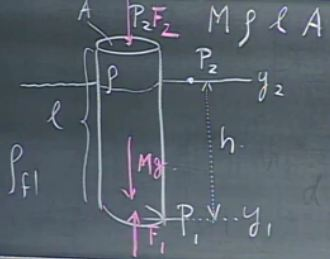
\includegraphics[scale=0.8]{Graphics/lec28_floating_cylinder}
\end{center}

There is a downwards force $F_2 = A P_2$ due to the weight of the air above the cylinder, and an upwards force $F_1 = A P_1$ due to the hydrostatic pressure. �n addition, there is a gravitational force $M g = A \ell \rho g$ downwards.

Via Pascal's law, $P_1 - P_2 = \rho_{fl} g h$.

In equilibrium, the forces on the cylinder must be balanced:

\begin{equation}
F_1 - F_2 - M g = 0
\end{equation}

If we multiply both sides of the Pascal's law equation by $A$, we find

\begin{equation}
A P_1 - A P_2 = A \rho_{fl} g h
\end{equation}

The left side here, $A P_1 - A P_2 = F_1 - F_2$, is known as the \emph{buoyant force}. The other side is the \emph{weight of the displaced fluid}: $A h$ is the volume of the the displaced fluid, times $\rho_{fl}$ gives us the mass, and times $g$ times us the weight.

This is a case of \emph{Archimedes' principle}, which can be stated as: ``the buoyant force on an emerged body has the same magnitude as the weight of the fluid which is displaced by the body''.

The story is that Archimedes was given the task to find out whether a crown made for his king was made of pure gold. He therefore wanted to measure the density of the crown -- but how does one measure the density of something without destroying it? The simple solution would be to measure the volume and the weight, and then calculate the mass and density from there. However, measuring the volume of such an irregularly shaped object with e.g. a meter stick is no easy task!

What he realized (according to the legend, when he noticed the water rise as he stepped into a bath) was that he could measure the volume by submerging the crown in water.\\
Silver has a lower density than gold, so if part of the crown was silver, for a given mass/weight, it would have to be slightly larger in volume. Measuring the weight is relatively easy, but even then, measuring a fairly small change in volume is still not easy, as the change in water level would be very small (probably less than 1 mm, depending on the container size etc.). Not only that, but there could be other factors causing trouble, such a surface tension, which may well make the difference completely impossible to measure.

What one can do is the following. First, we weigh the crown as per usual, perhaps using a spring, and find a weight $W_1 = V \rho g$, where $V$ is the volume of the crown.\\
Next, we submerge it in water, and weigh it there. Because of the buoyant force acting on the crown, its weight is less under water. (Its \emph{mass} is of course the same.)

In water, the weight is the original weight, minus the buoyant force $V \rho_{fl} g$, which is the weight of the displaced fluid of volume $V$. So we have

\begin{align}
W_1 &= V \rho g\\
W_2 &= V \rho g - V \rho_{water} g = W_1 - V \rho_{water} g
\end{align}

We can solve this to find

\begin{equation}
\rho = \frac{W_1}{W_1 - W_2} \rho_{water}
\end{equation}

and also

\begin{equation}
V = \frac{W_1 - W_2}{g \rho_{water}}
\end{equation}

All of the things needed to find $\rho$ was either known ($\rho_{water}$) or easily measurable (the weights), with rather high accuracy.

\subsection{Floating and icebergs}

I'm sure most of us have heard the expression ``that's just the tip of the iceberg''. There's a good reason for that expression, as we will see now.

Consider an iceberg of mass $M$, volume $V_{tot}$, density $\rho_{ice} = \SI{0.92}{g/cm^3}$, compared to $\rho_{water} = \SI{1}{g/cm^3}$.\\
Because it is floating, the buoyant force is equal in magnitude to $M g = V_{tot} \rho_{ice} g$. The buoyant force is given by the weight of the displaced water, $F_b = V_{sub} \rho_{water} g$, where $V_{sub}$ is the volume of the iceberg that is submerged, i.e. under water.

\begin{equation}
V_{tot} \rho_{ice} g = V_{sub} \rho_{water} g
\end{equation}
\begin{equation}
V_{tot} \rho_{ice} = V_{sub} \rho_{water}
\end{equation}

$g$ cancels. We can rearrange the equation:

\begin{equation}
\frac{V_{sub}}{V_{tot}} = \frac{\rho_{ice}}{\rho_{water}} = 0.92
\end{equation}

So the submerged volume is going to be 92\% of the total volume: 9/10 of the iceberg is under water, and we can indeed only see the tip of it from above water.

Going back to our cylinder from the beginning of the lecture, what is the condition for floating? We know already that the buoyant force must equal the weight, and we have already learned that the buoyant force is equal to the weight of the displaced water, $A h \rho_{fl} g$, where $h$ is the height of the part of the cylinder that is under water.\\
That must be equal to the weight of the cylinder, $A \ell \rho g$, so after cancelling $A$ and $g$ we have

\begin{equation}
h \rho_{fl} = \ell \rho
\end{equation}

However, $h < \ell$ must be the case: the amount submerged must be less than the total height, or it would be entirely underwater. With that condition, to balance the two sides out to be equal, it must also be the case that

\begin{equation}
\rho_{fl} > \rho
\end{equation}

Very simple, indeed. Things float if their density is smaller than the density of the fluid they are in. Note that the masses or weights don't matter: a small pebble, say a 2 mm radius ``rock'', will sink in water, because rock has a greater density than water. A 1 km radius iceberg, with a mass of over $10^{12}$ kg would float in water, however, since the density of ice is smaller than the density of water.

Let's now consider an interesting question. We are in a boat, in some small-ish reservoir of water, like a swimming pool. We have a large/heavy rock in the boat with us. If we throw this rock overboard, so that it sinks, will the water level in the pool go up, go down, or stay the same as it was when the rock was inside the boat?

When it is in the boat, the boat displaces extra water due to the weight of the rock, $W = V \rho_{rock} g$, which causes the water level to rise (compared to the rock not being there at all).\\
When it is in he water, it displaces water equal to the volume of the rock; the displaced water then has a weight $V \rho_{water} g$.\\
So which is greater? The rock's weight is $V \rho_{rock} g$, while the weight of the displaced water in case is $V \rho_{water} g$. The former is clearly greater, since the rock 's density is much greater than the density of water.

More water is therefore displaced when the rock is in the boat, and so the water level will go \emph{down} when it is instead in the water.

\subsection{Stability of immersed objects; balloons}

Consider a floating object, which has a center of mass not aligned with its geometrical center. Perhaps it's an iceberg with some rocks in it.

\begin{center}
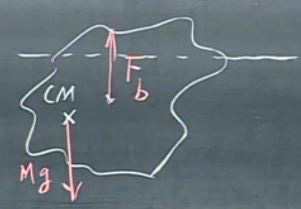
\includegraphics[scale=0.7]{Graphics/lec28_iceberg_torque}
\end{center}

Gravity acts at the center of mass, as usual, but the buoyant force does not! It acts at the center of mass \emph{of the displaced fluid}, which is this case will be to the right of the iceberg's center of mass. Therefore, these two forces create a counterclockwise torque, causing the object to rotate.

Just as we saw previously, with an object on a pin, it will rotate until these forces are vertically aligned, so that is no longer any net torque.\\
Also as we saw previously, there are two possible cases where this happens: one where the center of mass of the iceberg is \emph{above} the point of application of the buoyant force, which would be a case of unstable equilibrium, or the more stable case where it is \emph{below}.

This is then a very important issue in the construction of ships. If a ship were to have the center of mass above the point where the buoyant force is applied, it could very easily capsize (flip around upside down). The lower the center of mass is, the more stable a ship will be.

Next, let's have a quick look at balloons, specifically ones with light gases inside, such as helium. What is the condition for them to float and rise in air?\\
Well, the situation is really very similar to an object floating in water.

The balloon has a certain mass $M$, given by the mass of the gas inside $V \rho_g$ plus the mass of the ``rest'', i.e. the balloon itself (the rubber, perhaps a string, etc). It then has a weight $W_{balloon} = g(V \rho_g + M_{rest})$.\\
In order to rise, the buoyant force must be greater than this weight. The buoyant force is given by the weight of the displaced fluid -- and the fluid is air, here. $W_{air} = V \rho_{air} g$, so the condition is

\begin{align}
V \rho_{air} g &> V \rho_g g + M_{rest} g\\
V \rho_{air} &> V \rho_g + M_{rest}
\end{align}

It's clear, then, that $\rho_g < \rho_{air}$ must be the case. That is necessary, but not sufficient: it is sufficient only for a massless balloon. Since the rubber has a small mass, the density of the gas must be smaller by a margin wide enough to also carry that mass.

\subsection{Helium balloon in an accelerated frame}

We will now look at a second example involving helium balloons. I will shorten this section compared to the lecture, which should (as always) be watched anyway, especially as this is a demonstration.

In short: in the presence of air, a helium balloon will always move in the direction that opposes gravity. That includes perceived gravity, for example due to a rocket accelerating in outer space.\\
So say we have a sealed-off ``room'' somewhere in outer space, where the gravity due to the surrounding stars etc. is completely negligible. We accelerate this system, say ``upwards'' (as shown in a drawn figure, that is). We will perceive gravity in the opposite direction, which means we will fall down, as will the air inside the room. However, as the air will sink down due to its weight (which was zero prior to the acceleration), we will essentially end up with an atmosphere inside. The pressure will be higher near what has now become the floor, and smaller at the roof. Therefore, the helium balloon will rise towards the roof, in the \emph{same} direction of the acceleration.

So far, this is a bit strange perhaps, but it still appears reasonable, since acceleration creates perceived gravity, which we cannot really tell apart from ``regular'' gravity.\\
However, now consider doing this in a room here on Earth, only we accelerate it towards the right, rather than up.\\
We have a closed compartment filled with air; it indeed needs to be closed, since this effect relies on the pressure difference between the two sides.

If we hang an apple from a string, we know what will happen: accelerate the box towards the right, and the apple will resist this motion, and appear to lean to the left.\\
However, what if we have a helium balloon, attached to the floor via a string? Before we push, it will happily float and just sit there, trying to move opposite gravity, but being stopped by the downwards tension in the string. When we accelerate the box towards the right, the air inside this closed compartment ``falls'' towards the left. Again, a pressure difference is created, such that the pressure at the left side is greater than the pressure on the right side.\\
This causes a horizontal buoyant force, and the balloon will ``float'' and move \emph{towards the right}.

That is, unlike what we would expect any object to do, it moves \emph{forward}, along with the acceleration. This can also be replicated in a car, for example. Step on the gas, and the balloon will move forward, while the passengers are pushed back into their seats; slam the brakes, and the balloon will move backward, while everyone moves forward. Not very intuitive.

\subsection{Bernoulli's equation}

We will now show a rather fast derivation of Bernoulli's equation for incompressible fluids.

Say we have a flow between two different heights, with two different areas, pressures and fluid velocities, as follows:

\begin{center}
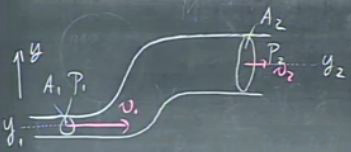
\includegraphics[scale=0.8]{Graphics/lec28_bernoulli}
\end{center}

Because the fluid is incompressible, the amount of fluid that passes though $A_1$ per unit time must be the same as the amount that passes through $A_2$ per unit time; that is, $A_1 v_1 = A_2 v_2$. For that reason, in this case, $v_1 > v_2$.

In the case where the fluid is static, $v_1 = v_2 = 0$, we could apply Pascal's law: $P_1 - P_2 = \rho g (y_2 - y_1) = \rho g h$, using the usual definition $y_2 - y_1 = h$.\\
This then implies that the pressure at $A_1$ is higher than the pressure at $A_2$, since it is at a lower level, which implies higher pressure.

We know $m g h$ as being a term of gravitational potential energy. However, $m$ divided by volume gives us density $\rho$; therefore, the above expression is in terms of gravitational potential energy per unit volume, $\displaystyle \frac{m g h}{V} = \frac{m}{V} g h = \rho g h$.\\
Since we can only equate quantities that have the same dimension, the dimension of pressure must be the same as energy per unit volume.

If we now consider the dynamic case, where the velocities come in to play, we also have kinetic energy to consider. We can then relate the kinetic energy per unit volume, $\displaystyle \frac{1}{2} \frac{m}{V} v^2 = \frac{1}{2} \rho v^2$, gravitational potential energy per unit volume $\rho g y$, and the pressures. The sum of these three terms must then remain a constant, via the conservation of energy.

\begin{equation}
\frac{1}{2} \rho v^2 + \rho g y + P = \text{constant}
\end{equation}

The above is one way of writing \emph{Bernoulli's equation}. Just as Pascal's law, this equation has some very interesting (and strange) properties.

Consider a tube that changes diameter (like above), but where the level $y$ stays constant. We still have an incompressible fluid of density $\rho$, and two areas $A_1$ and $A_2$, with pressures $P_1$ and $P_2$, respectively; the fluid has speeds $v_1$ and $v_2$ respectively at the two places, where $v_1 > v_2$, because as earlier, $A_1 v_1 = A_2 v_2$ must hold for a fully incompressible fluid.

Since we measure the pressure at the same height $y$, the total energy equation for both places contain a $+ \rho g y$ term, which then cancels. We can then simplify down the result, to arrive at

\begin{align}
\frac{1}{2} \rho v_1^2 + \rho g y + P_1 &= \frac{1}{2} \rho v_2^2 + \rho g y + P_2\\
P_1 + \frac{1}{2} \rho (v_1^2 - v_2^2) &= P_2\\
\end{align}

Because the non-pressure term is positive, it must be the case that $P_2 > P_1$. Very nonintuitive, to me -- I would absolutely have guessed that the pressure would be higher at $A_1$ where not only the velocity is greater, but the liquid seems to be more tightly packed... but that is not the case.

\subsection{Siphons}

Most of us have probably seen a siphon (or syphon) in action. We have a container of water that is at a height, and a hose (with a diameter much smaller than that of the container) going down below the container.

\begin{center}
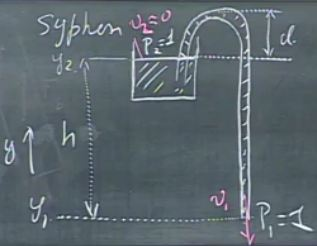
\includegraphics[scale=0.8]{Graphics/lec28_siphon}
\end{center}

$v_2$, the velocity of the liquid in the container, can be approximated as zero, if it is much larger than the diameter of the hose.\\
Both the top of the liquid in the container and the liquid flowing out is directly exposed to the atmosphere, so $P_1 = P_2 = 1$ atm. Therefore, in our conservation of energy equation, we lose the pressure terms. With that in mind, having different $y$ values this time, and $v_2 \approx 0$, we find, also using $y_2 - y_1 = h$,

\begin{align}
\frac{1}{2} \rho v_1^2 + \rho g y_1 &= \rho g y_2\\
\rho v_1^2 &= 2 \rho g (y_2 - y_1)\\
v_1 &= \sqrt{2 g h}
\end{align}

This is \emph{exactly} the velocity we would find for an object being accelerated down by gravity. When starting at 0 velocity and having fallen a distance $h$, an object in free fall has the velocity $\sqrt{2 g h}$. In other words, the siphoned liquid is acting as if it's in free fall.

That much may be intuitive, but the strange part is once the flow has begun, we can raise the hose up, i.e. increase $d$, up until the $\approx \SI{10}{m}$ limit discussed earlier (for water), as long as the end of the hose is below the container, and the liquid will keep flowing.\\
We need to get it started manually, though, but sucking on the free end. Once that's done, the entire container will empty all by itself.

\subsection{A few quick experiments}

Consider a funnel, with a ping-pong ball inside:

\begin{center}
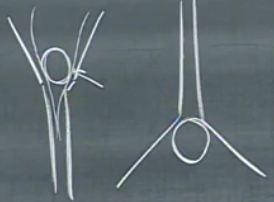
\includegraphics[scale=0.8]{Graphics/lec28_funnel}
\end{center}

First, we hold it upright. If we try to blow and get the ball to move upwards, what will happen? The opposite of what we might think: the harder to blow, the more the ball is sucked down. According to the Bernoulli principle, the pressure is lower in the thin part, where the velocity is high. Therefore, there is an underpressure there, and the ball is sucked down more than it is blown upwards.

The effect is strong enough that we can do the experiment upside down, and hold it in place (for a short time, at least) merely by blowing out, as the second figure above shows.

Next, we have an air pump, blowing to keep a ping-pong ball floating in mid-air:

\begin{center}
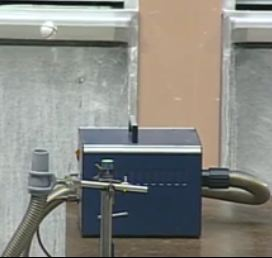
\includegraphics[scale=0.8]{Graphics/lec28_air_pump}
\end{center}

It is held up for reasons to do with turbulence, which is more complex than we can discuss here. However, Bernoulli's principle comes into play in another way: the stability. While it's obviously difficult to show this in a still image, the ball wobbles back and forth, but never falls out. Even when the hose is tilted perhaps 10-20 degrees, the system is still stable. This stability is because of Bernoulli's principle.

\begin{center}
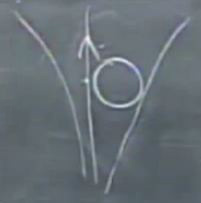
\includegraphics[scale=0.6]{Graphics/lec28_divergence}
\end{center}

The air is blowing faster near the center, as it is diverging away (the area is becoming larger, so the velocity goes down, as we saw earlier).\\
Therefore, the pressure is the lowest near the center, and when the ball moves away, it is being sucked back in by the lower pressure.

Finally, the professor demonstrates what happens if you fill a glass half-way, put a piece of cardboard (or some paper similar to a postcard in thickness, perhaps) over the top, and then turn it upside down. The liquid will tend to stay in place even upside down, with no support, so not only is the paper is held up against gravity, the liquid is as well.\\
This happens because air pressure is acting to push the paper up, stronger than gravity is pulling the water down.\\
There are other things at play too, though, including surface tension. I have not been able to find a fully satisfactory explanation of this, even though it seems so simple.

For example, why does this not happen when you simply turn the glass upside down, without the paper? Clearly, the paper isn't increasing the air pressure; if the air pressure can support the liquid via the paper, it must obviously be able to support the liquid itself, too! So why does the water simply run out, as we would expect intuitively, but perhaps not expect considering air pressure?

The explanation appears to be quite a bit beyond this course, in Rayleigh-Taylor instability. If the water surface could be \emph{perfectly} flat, it appears that it would indeed not fall out, though achieving this in practice is clearly either extremely difficult or plain impossible.

\end{document}